\section{Design and Implementation}
\label{sec:design}

In this section, we explain how the use the Markov chain as a mean for modelling occupancy data. By predicting the future of occupancy of a zone\footnote{A zone is an open or closed part of a building whose HVAC system is controlled by a single sensor.}, an intelligent system can tune conditioning parameters gradually to reflect the predicted changes in time.

\subsection{The Markov Chain Model}
The prediction of the temporal dynamics of the occupancy in a zone is carried out using a Markov Chain (MC).  It represents the chain of states which a process goes through and is usually defined as a process which can be observed at a discrete set of times.  To design our observed data to easily fit the MC model, the number of occupants in each zone of the building is taken, and a threshold and a simple state is assigned to each observation after the threshold.

For example, let the number of zones be 3, and the occupancy in each zone be based on a threshold vector $(say [0, 5, 10, 15])$.  This assigns states like \\
${(E)mpty,  (F)ew,  (A)verage,  (C)rowd} $ to each zone.  i. e if in a zone the observed number of occupants (N) is zero then a state (E) is assigned to the zone.  Similarly, if $N > 0 $ and $N <= 5$, then the zone is assigned the state (F), for $N > 5 $ and $N <= 10$ ,  the state is (A) and so on.  For a sample observed occupancy data of the building with 3 zones occupancy data at time t, their corresponding state is $[8,.22, 0] \Leftrightarrow [F,  C,  E]$ .

Using the occupancy distribution at any time ${t}$ and the derived state vector, the state vector for time ${t + \triangle t}$  is predicted.  The predicted state vector for ${t + \triangle t} $,. allows  the prediction of zones that are likely to be more or less occupied.  A transition matrix is used to represent the probability of the transition from one state to another.  It is a two dimensional matrix encompassing the probability of all possible transitions  and refers to a square table with dimensions [Number of states X Number of states].   The element of the matrix at any location (i, j) is the probability of transition from $i^{th}$ state to $j^{th}$ state which is designated as $p _ {ij}$.   Figure \ref{fig:states} explains the state transitions drawn from equation \ref{equ:1} and the corresponding transition matrix of the three states representing the number of occupants in a building.



\begin{figure}[!ht]
\centering
\resizebox{3.4in}{!}{%
\begin {tikzpicture}[-latex ,auto ,node distance =4 cm and 5cm ,on grid ,
semithick ,state/.style ={ circle ,top color =white , bottom color = processblue!20 ,
draw,processblue , text=blue , minimum width =1cm}]
\node[state] (C){$E$};
\node[state] (A) [above left=of C] {$F$};
\node[state] (B) [above right =of C] {$C$};
\path (A) edge [loop left] node[left] {$0.4$} (A);
\path (B) edge [loop right] node[left] {$0.1$} (B);
\path (C) edge [loop below] node[left] {$0.2$} (C);
\path (C) edge [bend left =25] node[below =0.15 cm] {$0.5$} (A);
\path (A) edge [bend right = -15] node[below =0.15 cm] {$0.3$} (C);
\path (A) edge [bend left =25] node[above] {$0.3$} (B);
\path (B) edge [bend left =15] node[below =0.15 cm] {$0.5$} (A);
\path (C) edge [bend left =15] node[below =0.15 cm] {$0.3$} (B);
\path (B) edge [bend right = -25] node[below =0.15 cm] {$0.4$} (C);
\end{tikzpicture}}
 \caption{ State diagram of Markov Chain with states Empty, Few or Crowded} \label{fig:states}
\end{figure}


\[
P=
  \begin{bmatrix}
  &Empty & Few & Crowded \\
Empty & 0.2&0.5&0.3\\
Few & 0.3&0.4&0.3\\
Crowded& 0.4&0.5&0.1\\
  \end{bmatrix}
\]


\begin{equation}
\begin{split}
\label{equ:1}
P( X _ {t+1} = s _ {t+1} | X _ t = s _ t ,  X _ {t-1} = s _ {t-1},
\ldots ,  X _ 0 = s _ 0 ) \\
= P( X _ {t+1} = s _ {t+1} | X _ t = s _ t )
\end{split}
\end{equation}

In P, all elements represent the probability of the transition from one state to another, including the same state.  For example, element $(2, 1)$ is the probability $P{21} = 0.4$ of the transition from the 2nd state which is (Few) to state 1 (Empty).  One of the main properties of the transition matrix is that the sum of all elements in any row equals 1.

\begin{equation}
\begin{split}
\label{equ:2}
\sum_{i=const, j=0}^{k-1} P_{i, j} = 1,   \\
 \text{Where k is the number of states}
\end{split}
\end{equation}

For any number of observations, the MC model can be easily applied to describe a single time step of event, i. e.  considering the present state (at t) the states at an immediate future time-step at ${t  + \triangle t}$  is described by the transition matrix.   In order to understand the probability of the transition from the present state to any particular state after n time-steps ${n \triangle t}$, then  we will use the following simple equation.

\begin{equation}
 \centering
\label{equ:4}
P_{ij}^{(n)} = \sum_{k=1}^{M} P_{ik} P_{kj}
\end{equation}

\subsubsection{Learning the Transition Matrix}
The entity that we are modelling is a dynamic process subject to changes with time. The transition matrix is built with occupancy data collected over time, in half an hour increment, in all registered zones.  For each zone, the probability of a particular transition (matrix element) is calculated by finding the ratio of the number of this transition with respect to the total number of transitions occurring.
\begin{equation}
 \centering
\begin{split}
\label{equ:5}
P_{ij} = n_{ij} \/ \sum_{k=1}^{M}  n_{ik} ,  \\
\text{Where m is the possible number of transitions}
\end{split}
\end{equation}


After building the transition matrix with a suitably large data set, it becomes possible to identify similar patterns in a new set of observations.

 Figure \ref{fig:occupflow} below shows the layout of a hypothetical office and the distribution of 7 Kinect sensors on its floors.
\begin{figure}[!ht]
  \centering
 	  	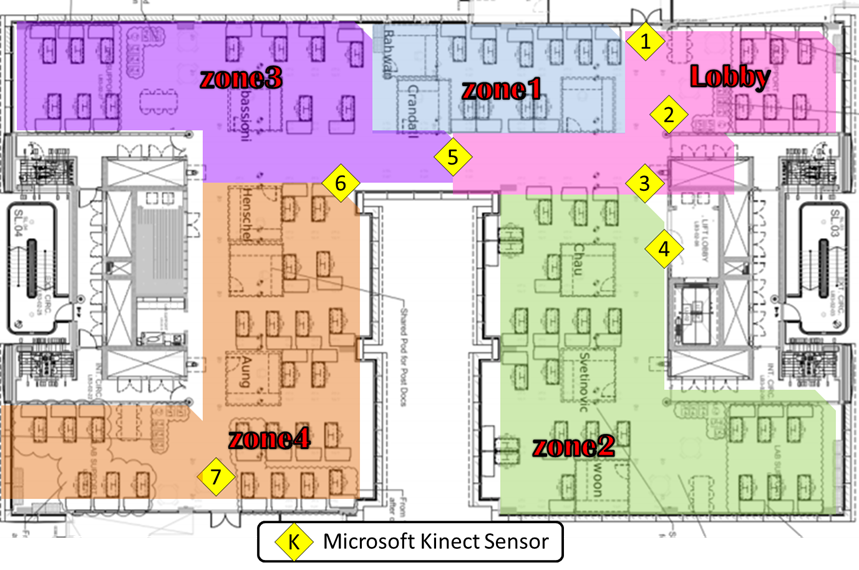
\includegraphics[width=0.9\columnwidth]{./images/numberofkinect.png}
  \caption{Distribution of 7 Kinect sensors on a building's floor layout.}\label{fig:occupflow}
\end{figure}

A log file is created in a format of the Table below \ref{table:logfile}:
 \begin{center}
\begin{table}[!ht]
  \centering
  \begin{tabular}{*6c}
08/10/2013& 22:51:30& IN:& 0 &OUT:& 1\\
08/10/2013& 22:51:31 &IN: &0 &OUT:& 2\\
08/10/2013 &23:30:30& IN: &0& OUT: &3\\
08/10/2013& 23:58:15 &IN:& 0 &OUT:& 4\\
09/10/2013 &05:17:21& IN: &1 &OUT:& 4\\
09/10/2013 &06:35:36 &IN:& 2& OUT:& 4\\
09/10/2013 &06:36:20& IN:& 2& OUT:& 5\\
09/10/2013 &07:09:11& IN: &3& OUT:& 5\\
09/10/2013 &07:15:04 &IN:& 3& OUT:& 6\\
09/10/2013 &07:25:46& IN:& 4& OUT: &6\\
\end{tabular}
\caption{Output log file for mobility tracking with exact timestamp at each sensor virtual gate.}
\label{table:logfile}
\end{table}
 \end{center}

This data is then parsed and converted into a different format in order to compute the effective occupancy of a zone.  The new format has 48 half hour time slots a day, and on each time slot the net people count is logged.

After counting the differences between the inflow and outflow of occupants, along with the previous estimate of the occupancy of each zone and the corresponding sensor gates, the net occupancy of each zone at a given time slot is calculated.

This data is related to the threshold vector [0, 5, 10, 15] and assigned one of the four states {E, F,  A, C}.   This data is referred to as the state matrix in \ref{table:stateslog}.
\begin{table}
  \centering

   \begin{tabular}{*5c}
Lab1&Lobby&Lab2&Lab3&Lab4\\
E&F&E&E&E\\
E&E&C&E&E\\
E&F&E&M&F\\
. &. &. &. &. \\
. &. &. &. &. \\
. &. &. &. &. \\
\end{tabular} \caption{Zone condition from occupancy data table.} \label{table:stateslog}
\end{table}

The number of possible states that can be observed in the building is equal to \ref{equ:6}
\begin{equation}
\label{equ:6}
\text{ ${(number of individual states)}^{(number of zones)}$}
\end{equation}

The total number of possible states of the building in this case is 1024,  from all 5 zones conditions of different element combinations of {E, F, A, C} ranging from {(E, E, E, E, E)}, {(E, E, E, E, F)}, {(E, E, E, E, M)} to {(C, C, C, C, C)}.

The transition matrix of size  [1024 X 1024], is then trained using the data above and the equation \ref{equ:5}, by counting the number of times a transition takes place divided by the total number of transitions.  There is a possibility that the input data set is not exhaustive in nature.  The transition matrix that is obtained is normalized row-wise to make the property in the equation true\ref{equ:2}.

After the matrix is trained, the implementation of the prediction system is simple and straightforward.  With new observations as the state matrix is updated with time, for any new row obtained, the state vector is taken say ({E, E, E, E, F}) and a one-time step prediction is made by finding the row number in the transition matrix which represents the state vector (row 2) and the column number with the maximum probability value is taken.  The state vector corresponding to the column number is the next predicted state of the building.

\subsection{Sample Model}

To understand how the problem is solved in-depth,  a sample date is observed and used to train the transition matrix. Let us consider a building floor consisting of two zones.  As the sensors observe the occupancy of each zone, with people entering or exiting any zone data is logged.  After parsing these log files, it is possible to obtain the occupancy of each zone in 48 time slots a day.   Table \ref{table:eee} formed for 12 slots  shown below is an example.
\begin{table}[!ht]
  \centering
      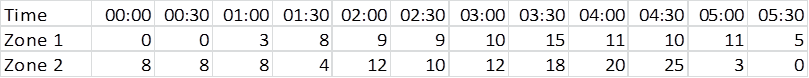
\includegraphics[width=0.9\columnwidth]{./images/t1.png}
  \caption{Example of occupancy data for two zones in a building.}\label{table:eee}
\end{table}

For thresholds, the occupancy matrix with a threshold vector [0, 5, 10] and assigning individual states {E, F, A, C} we get the table below \ref{table:vectort}:
\begin{table}[!ht]
  \centering
  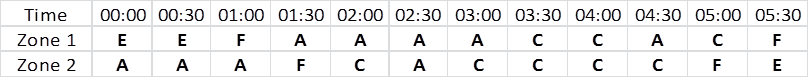
\includegraphics[width=0.9\columnwidth]{./images/t2.png}
  \caption{Representation of occupancy data, with transition condition.}\label{table:vectort}
\end{table}

For this problem, there are 16 possible combined states called state vectors.  The transition matrix that is formed is of size [16 x 16].  From the above table, we see that there are 11 transitions.  In a [16 x 16] matrix of zeroes,  for each transition observed the row number corresponding to the initial state vector is taken and the column number corresponding to next state vector is taken,  and the element at (row-number,  column-number) is incremented by 1.

Normalizing the transition matrix along the row, we get Table \ref{table:tmp} below:
\begin{table}[!ht]
  \centering
    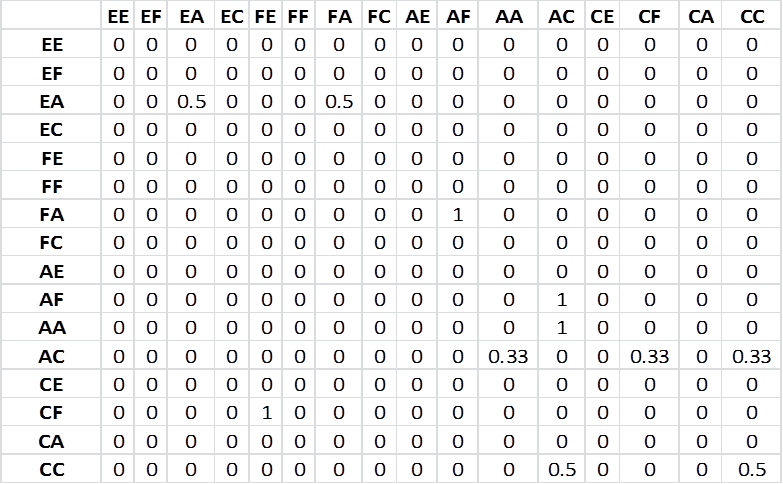
\includegraphics[width=0.9\columnwidth]{./images/t4.png}
  \caption{The transition probability between states.}\label{table:tmp}
\end{table}

The matrix has many empty rows, which shows that it is inadequately trained. After finding the transition matrix, the system is ready to predict future occupancy.  For an observation of [zone 1, zone 2] equal to say [8, 13], we get the state vector [A, C].  The next state of the building can then be obtained by taking the row MC and finding the index of the maximum element in the row, which is CA, with probability 0. 0929.



\subsection{Kinect-based Occupancy Counter software}
Our  Occupancy Counter software is written using Microsoft Visual $C\sharp$ 2010,  project WPF application programmed using $C\sharp$ and XML languages.  OS used is Windows 7 with Kinect Studio v. 1. 7. 0 and Developer Toolkit Browser v. 1. 7. 0 installed.  Both type of Kinect is used and tested to be running on our software,  Xbox Kinect and Kinect for windows.  The software,  should be run in windows 7 or above,  with pre-installation of Kinect sensor drivers \emph{(shortly by installing Kinect SDK)}.

 \begin{figure}[!ht]
  \begin{center}
	  	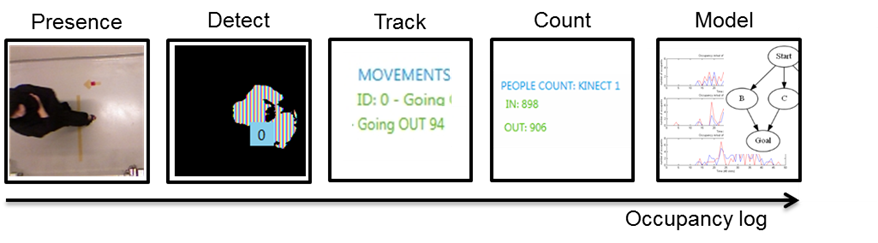
\includegraphics[width=0.9\columnwidth]{./images/112200.png}
  \end{center}
  \caption{Human detection,  tracking, counting and analysis.}
\end{figure}

\begin{enumerate}
  \item \textbf{Kinect initialization start:} This function will look up for any connected Kinect devices to your computer.  If no device is connected: a box message will appear to inform you about this fact.  The software display both RGB and Depth image,  Figure \ref{fig:guioverview} show the GUI of our software.

     \begin{figure}[!ht]
  \begin{center}
	  	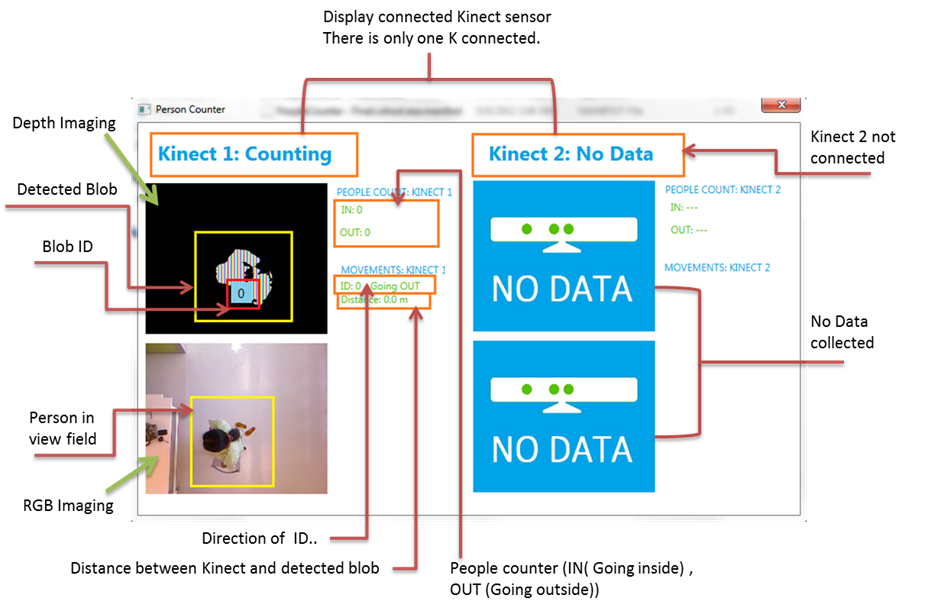
\includegraphics[width=0.9\columnwidth]{./images/swm.png}
  \end{center}
  \caption{Overview of the GUI of our Kinect-based Occupancy Counter x.}
  \label{fig:guioverview}
\end{figure}
\item \textbf{Capture frame events}: As part of the initialization,  it makes sure that both RGB and Depth imaging are captured.
ColorImageFrameReadyEventArgs:	The event arguments provided in a KinectSensor. ColorFrameReady event when a frame of color data is ready.
\item \textbf{Depth camera feed generator:} Contains a per-frame buffer for depth data streamed out of a sensor.  Also provides access to the dimensions and format of the data in addition to mapping between skeleton and color coordinate spaces.  Once our Depth imaging is ready, we can start tracking blobs and draw markers.
\item \textbf{Generate Markers :} This draws a rectangle blue box  with unique ID of people that is used is temporarily  for the detection of multiple subjects passing in the field view.

\end{enumerate}


\begin{figure} [!ht]
  \begin{center}
	  	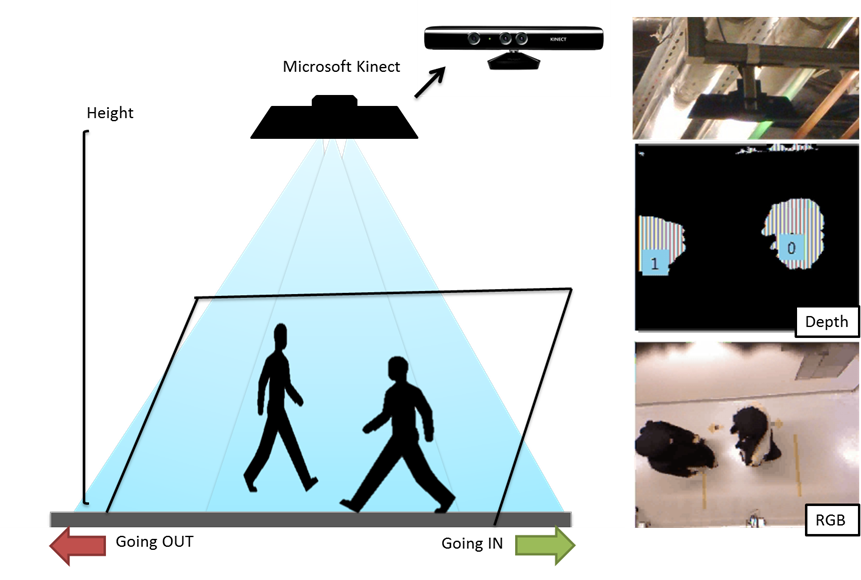
\includegraphics[width=0.9\columnwidth]{./images/minisys.png}
  \end{center}
  \caption{The architecture of our tracking system}\label{fig:minisys}
\end{figure}

People tracking through the Kinect sensor can be done using two methods:people tracking via human posture and an existing skeletal tracking by MSDN library. Both methods are implemented into our software to help us draw a fair comparison.

\subsection{Real World test-bed}
A human mobility detection system was implemented through a whole floor of a laboratory building. Since there might be difficulties and challenges in any deployment system, the sensors cover the most important parts/directions of lab areas that most students use. 7 Kinect sensors implemented in an I-smart laboratory at Masdar institute, the lab is occupied by 9 professors each supervising around 6-8 students.

\begin{figure} [!ht]
  \begin{center}
	  	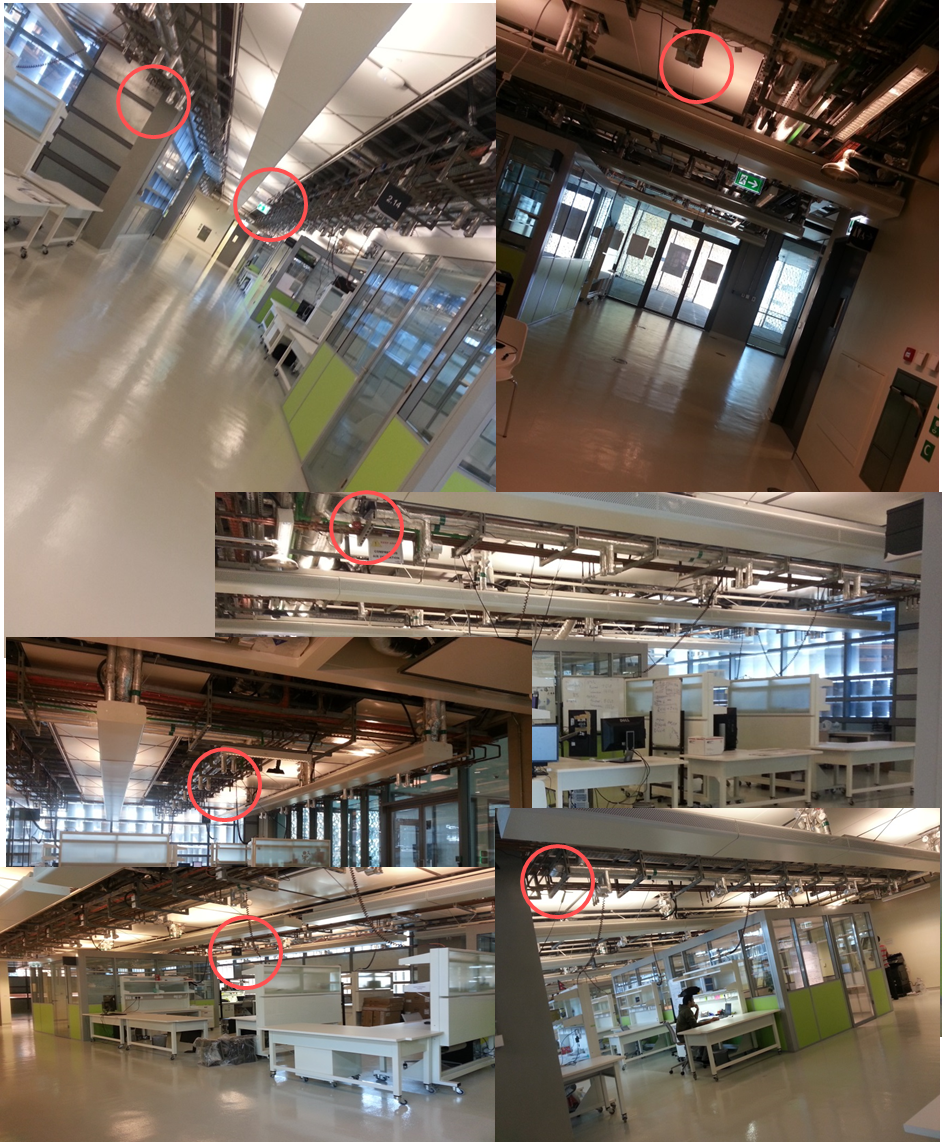
\includegraphics[width=0.9\columnwidth]{./images/realworld.png}
  \end{center}
  \caption{The real world test-bed }\label{fig:tstbd}
\end{figure} 